\subsection{Explain different physical mechanisms, which can lead to molecular binding between atoms. Which type of molecular potentials can be expected? Discuss approximations to these potentials.}


Generelt er der to mekanismer, som gør at molekylære bindinger opstår mellem to neutrale atomer og lader dem sammen danne et stabilt molekyle. Vi vil se, at disse både afhænger af de specifikke atomer, men også af afstanden mellem de to kerner $R$, som set på \cref{fig:Q19_ReasonsForMolecularBinding}: Kemiske bindinger, som opstår idet, at atomernes orbitaler overlapper, og multipolvekselvirkningen, som opstår idet, at atomers opførsel som magnetiske dipoler vekselvirker med hinanden. Af kemiske bindinger vil vi kigge på de \textsf{kovalente bindinger}, og af multipolvekselvirkningerne vil vi kigge på \textsf{Van der Waals-bindinger}.\footnote{
    Ydermere findes der også følgende bindingstyper:
    \begin{itemize}
        \item \textsf{Ionbindinger} (eng. ionic bond) opstår mellem positive og negative ioner, hvis der sker en udveksling af en (eller flere) elektroner fra atom A til  således, at atom A har en lavere elektrondensitet og B en større densitet.
        \item \textsf{Hydrogenbindinger} (eng. hydrogen bond) opstår idet at der sker en ladningsforskydning mellem atomet X, som hydrogen er bundet til, og hydrogen selv, så f.eks. for vand ($\text{H}_2\text{O}$, hvor elektroner bindes tættere til oxygen end hydrogen, hvorfor der forekommer en polarisation af vandmolekylet. Hydrogen ser altså mere positiv ladning end negativ, da dens elektronsky er forskubbet mod oxygen. Et andet vandmolekyle vil derfor have lyst til at binde sig med en hydrogenbinding til det første vandmolekyle således, at det svagt negativt polariseret oxygen-atom fra det andet vandmolekyle binder sig med det svag positivt polariserede hydrogen-atom fra det første molekyle. For bindinger mellem hydrogen og et andet alkalimetal er polarisationen omvendt, så hydrogen bliver negativt polariseret, da alkalimetaller binder elektronerne svagt.
    \end{itemize}
}

\begin{figure}[!h]
    \centering
    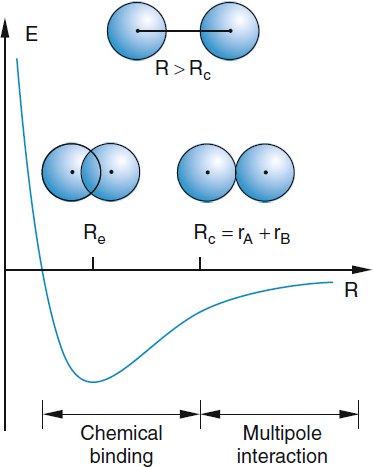
\includegraphics[width=0.45\textwidth]{Q19/images/ReasonsForBinding.PNG}
    \caption{Kemisk binding med overlab mellem atomorbitalerne er vigtig for $R < R_c$, hvor $R_c = r_A + r_B$ idet at $r_i$ er radius af atom $i$. For $R > R_c$ dominerer multipolvekselvirkningen (eng. multipole ineraction). $R_e$ er ligevægtsafstanden mellem atomerne.}
    \label{fig:Q19_ReasonsForMolecularBinding}
\end{figure}


\paragraph{Kovalente bindinger:} De kovalente bindinger opstår, når $R < R_c = \braket{r_A} + \braket{r_B}$, altså når afstanden mellem kernerne er mindre end summen af den gennemsnitlige atom radius af de to atomer. Dette er tilfældet, når de to atomers orbitaler overlapper. I dette tilfælde er der to effekter, som begge har indvirkning på bindingsenergien af molekylet (ved ligevægtsafstanden $R_e$).\\

\underline{Deling af valenselektroner:} Den første effekt, som har indvirkning, er den rummelige omstrukturering af valenselektronernes ladningsfordeling. Elektrontætheden bliver større inde mellem de to kerner, hvilket resulterer i en elektrostatisk tiltrækning mellem de positive kerner og denne negative elektrontæthed mellem kernerne. I kemisk bundne atomer deles én eller flere valenselektroner fra hvert atom i en fælles molekyleorbital. Dette er også beskrevet i \textsf{LCAO-approksimationen}, hvor den molekylære orbital er dannet af en linearkombination af atomorbitaler (eng. \textbf{L}inear \textbf{C}ombination of \textbf{A}tomic \textbf{O}rbitals).\\

\underline{Ombytningsvekselvirkning (eng. exchange interaction):} Den anden effekt er, at molekyleorbitalen har en større rummelig udstrækning end atomorbitalerne, hvilket øger den rummelige usikkerhed for elektronerne, hvorved deres gennemsnitlige impuls $\braket{|p|}$ mindskes ifølge Heisenbergs usikkerhedsprincip, og dermed også deres kinetiske energi $\braket{E_\text{kin}} = \braket{p^2}/(2m)$. Denne effekt kaldes ombytningsvekselvirkningen idet, at elektronerne i atomorbitalerne fra LCAO-approksimationen kan ombyttes, da de er identiske og dermed ikke kan skelnes i den fælles molekyleorbital.\\

Disse effekter leder sammen for stabile molekylære tilstande til et minimum i den potentielle energi $E(R)$ \footnote{Siden den potentielle energi indeholder den gennemsnitlige kinetiske energi af elektronerne.}. For afstande mindre end $R_c$ overlapper atomorbitalerne altså og danner molekyleorbitaler, hvor elektronerne deles mellem atomerne.

Betragter vi $H_2^+$, hvis bølgefunktioner kan findes ved LCAO-approksimationen, så kan man af \cref{fig:Q19_PotentialCurvesForSymmetricAndAntisymmetricWaveFunctionH2} se, at den symmetriske bølgefunktion lader et minimum eksistere i potentialet fra elektronerne, som kernerne mærker, hvilket den asymmetriske bølgefunktion ikke gør. Derved vil der være mulighed for molekylære bindinger, hvis atomerne har symmetriske bølgefunktioner og ikke asymmetriske.

\begin{figure}[!h]
    \centering
    \begin{subfigure}[t]{0.40\textwidth}
        \centering
        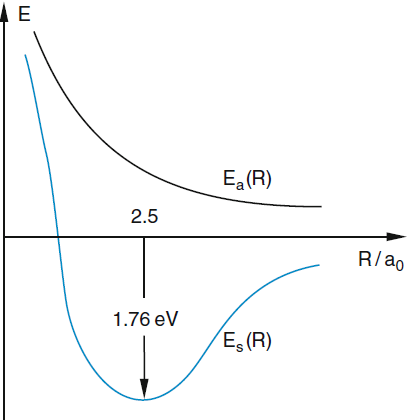
\includegraphics[width=.9\columnwidth]{Q19/images/PotentialCurvesForSymmetricAndAssymetricWaveFunctionH2.PNG}
        \caption{Potentialer.}
        \label{fig:Q19_PotentialCurvesForSymmetricAndAntisymmetricWaveFunctionH2}
    \end{subfigure}
    \hfill
    \begin{subfigure}[t]{0.45\textwidth}
        \centering
        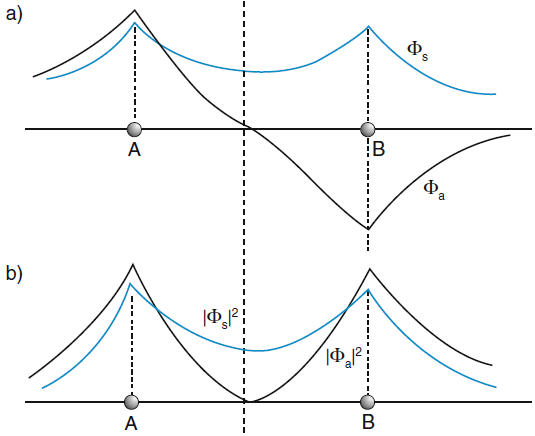
\includegraphics[width=\columnwidth]{Q19/images/SymmetriskOgAntisymmetriskBoelgefunktionForH2.PNG}
        \caption{a) $\psi^{A,S}$. b) $|\psi^{A,S}|^2$.}
        \label{fig:Q19_SymmetricAndAntisymmetricWaveFunctionsAndTheirProbability}
    \end{subfigure}
    \caption{Symmetrisk og antisymmetrisk bølgefunktion for $\text{H}_2^+$.}
    \label{fig:Q19_SymmetricAndAntisymmetricWaveFunctionsOfH2PlusIon}
\end{figure}


\paragraph{Van der Waals-bindinger:}